\chapter{Project Phases}
\label{chap:phases}

This chapter describes the project phases used in the planning and development of SitaWare Civilian.

Figure \ref{fig:project_phases} shows the six phases through which the system is to be developed. Furthermore, the figure contains the deliverables for the phase specific reviews. 

\begin{figure}[H]
\centering
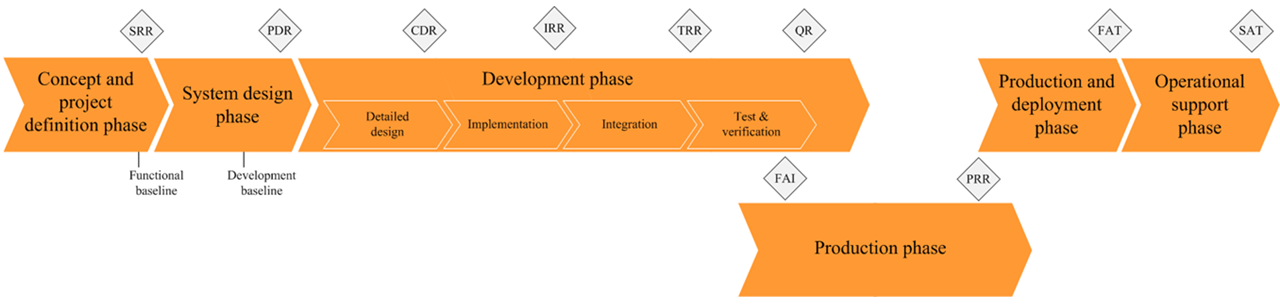
\includegraphics[width=0.95\textwidth]
{Billeder/project_phases/project_phases.PNG}
\caption{Project phases.}
\label{fig:project_phases}
\end{figure}


\paragraph{Concept and project definition phase}
This is the initial phase of the project and defines the problems and needs presented by the customer. By inspecting the needs, requirements to the system are identified. Furthermore, test methods for the defined requirements are specified. The phase ends with a system requirement review(SRR) between the development team and the customer. 

Deliverables:
\begin{enumerate}
\item[•] Time plan
\item[•] System Requirement Specification(SRS)
\item[•] Concept of Operations(CONOPS)
\item[•] Traceability matrix
\end{enumerate}


\paragraph{System design phase}
In this phase a plan for the conduct of the project is created. The plan covers what, by whom and when the different project elements are carried out. Furthermore, a preliminary design description is produced to close the gap between the requirements and the design phase, by clarifying the high-level design concept, which will implement the requirements in the SRS. The phase ends with a preliminary design review(PDR) between the development team and the customer. 

Deliverables:
\begin{enumerate}
\item[•] System Engineering Management Plan(SEMP)
\item[•] Preliminary Design Description(PDD)
\end{enumerate}


\paragraph{Development phase}
In this phase the actual product is designed, implemented, integrated and tested. The development phase consists of four subphases, each with their review: 
\begin{enumerate}
\item[•] \textbf{Detailed design:} \\
In this subphase the detailed design for the entire system is manufactured. The subphase ends with a critical design review(CDR) between the SW/HW designers and developers of the development company/companies.

\item[•] \textbf{Implementation:}\\
In this subphase the modules from the detailed design document(DDD) are implemented through SW classes and HW modules. The subphase ends with an internal integration readiness review(IRR) between the developers of the different interfacing modules.

\item[•] \textbf{Integration:}\\
In this subphase the developed HW/SW modules from the implementation subphase are put together to form the complete system. The subphase ends with a test readiness review(TRR) between the developers and the testers.

\item[•] \textbf{Test and verification:}\\
In this subphase the complete system is tested and verified according to the acceptance test in the SRS document(not written in this draft). The subphase ends with a qualification review(QR) between the customer and the development company. 
\end{enumerate}

The following deliverables form the basis of the related reviews:
\begin{enumerate}
\item[•] Detailed Design Description(CDR)
\item[•] Minutes of SubContractor Meeting(CDR)
\item[•] Integration Plan(IRR)
\item[•] System Test Description(TRR)
\item[•] Test Results Description(QR)
\end{enumerate}


\paragraph{Production phase}
In this phase a production plan and production schedule is prepared. The plan includes agreements with suppliers and a precise estimate of the economic aspects of production. Partway through the production phase the first factory produced item of the system is created and a first article inspection(FAI) is carried out, where minor corrections of the product are still possible without critical economic consequences. The phase ends with a production readiness review(PRR) between the production managers and the project management. The purpose of the PRR is to ensure that the project is on schedule for completion and ready to
go into production. No significant manufacturing may take place until after the PRR is successfully completed.


\paragraph{Production and deployment phase}
In this phase the product is put into mass production. This phase includes a factory acceptance test(FAT) performed by testers from, or hired by, the development company. The test is made to insure proper system functionality before shipping to a client. Time spent doing a proper FAT will lead to fewer problems when the equipment is installed on the site.


\paragraph{Operational support phase}
The last phase consists of system support according to the SRS document and a site/sea acceptance test(SAT). The SAT is carried out by one or more of the developing company's supporters at the client's site in cooperation with the client, to ensure proper installation and functionality. 
